\documentclass[10pt, compress]{beamer}
\usetheme[conference=AUG Monday,venue=Remote, date=29/05/2017, titleprogressbar, logo=RFX-logo]{Eurof}
\usepackage{listings,amsmath,multimedia, amssymb}
\usepackage{../beamerclass/tangocolors}
\usepackage{../beamerclass/rfxcolor}
% for drawing
\usepackage{pgf}
\usepackage{tikz}
\usetikzlibrary{arrows,shapes,backgrounds}
\usepackage{../beamerclass/onimage}
\usepackage[export]{adjustbox}
\usepackage{bm}
% for font
\usepackage[absolute,overlay]{textpos}
  \setlength{\TPHorizModule}{1mm}
  \setlength{\TPVertModule}{1mm}

\usepackage[style=nature,citestyle=authoryear-comp,defernumbers=true,maxnames=2,firstinits=true,
uniquename=init,backend=bibtex8,arxiv=abs,mcite]{biblatex}
\bibliography{biblio}
\renewcommand*{\bibfont}{\footnotesize}
\renewcommand*{\citesetup}{\footnotesize}
\usepackage[export]{adjustbox}
\makeatother
\mode<presentation>
\makeatletter
% add a macro that saves its argument
\newcommand{\footlineextra}[1]{\gdef\insertfootlineextra{#1}}
\newbox\footlineextrabox
% for reducing font on a single slide
\newcommand\Fontvi{\fontsize{8}{7.2}\selectfont}
\title{{\small Topic 21: Filamentary transport in high-power H-mode conditions and in no/small-ELM regimes to predict heat and particle loads on PFCs for future devices }}
\date{29 May 2017}
\author[Topic 21 Scientific Team]{N. Vianello for the Topic 21 Scientific Team}
\begin{document}
\tikzstyle{every picture}+=[remember picture]
\maketitle
\begin{frame}{Scientific team}
  \begin{center}
N. Vianello, D. Carralero, Z. Wei, J. Madsen, K. McClements,
M. Agostini, M.Spolaore, D. Aguiam, E. Wolfrum, J. Vicente,
L. Florian, E. Seliunin, J. Galdon-Quiroga, C. Ionita, S. Costea ...
  \end{center}
\end{frame}
\begin{frame}{Objective of Week 21 campaign}
  \begin{itemize}[<+-|alert@+>]
    \item Compare divertor/midplane fueling effect on filamentary
      transport and profiles without cryo-pumps
    \item Compare profiles with the same fueling with/without cryopums
    \item Determine an H-Mode with the cryopumps matching similar
      divertor pressure and SOL profiles
  \end{itemize}    
\end{frame}
\begin{frame}{Compare divertor/midplane fueling}
\Fontvi
  \vspace{-1cm}
\begin{columns}
  \begin{column}{0.65\textwidth}
    \centering{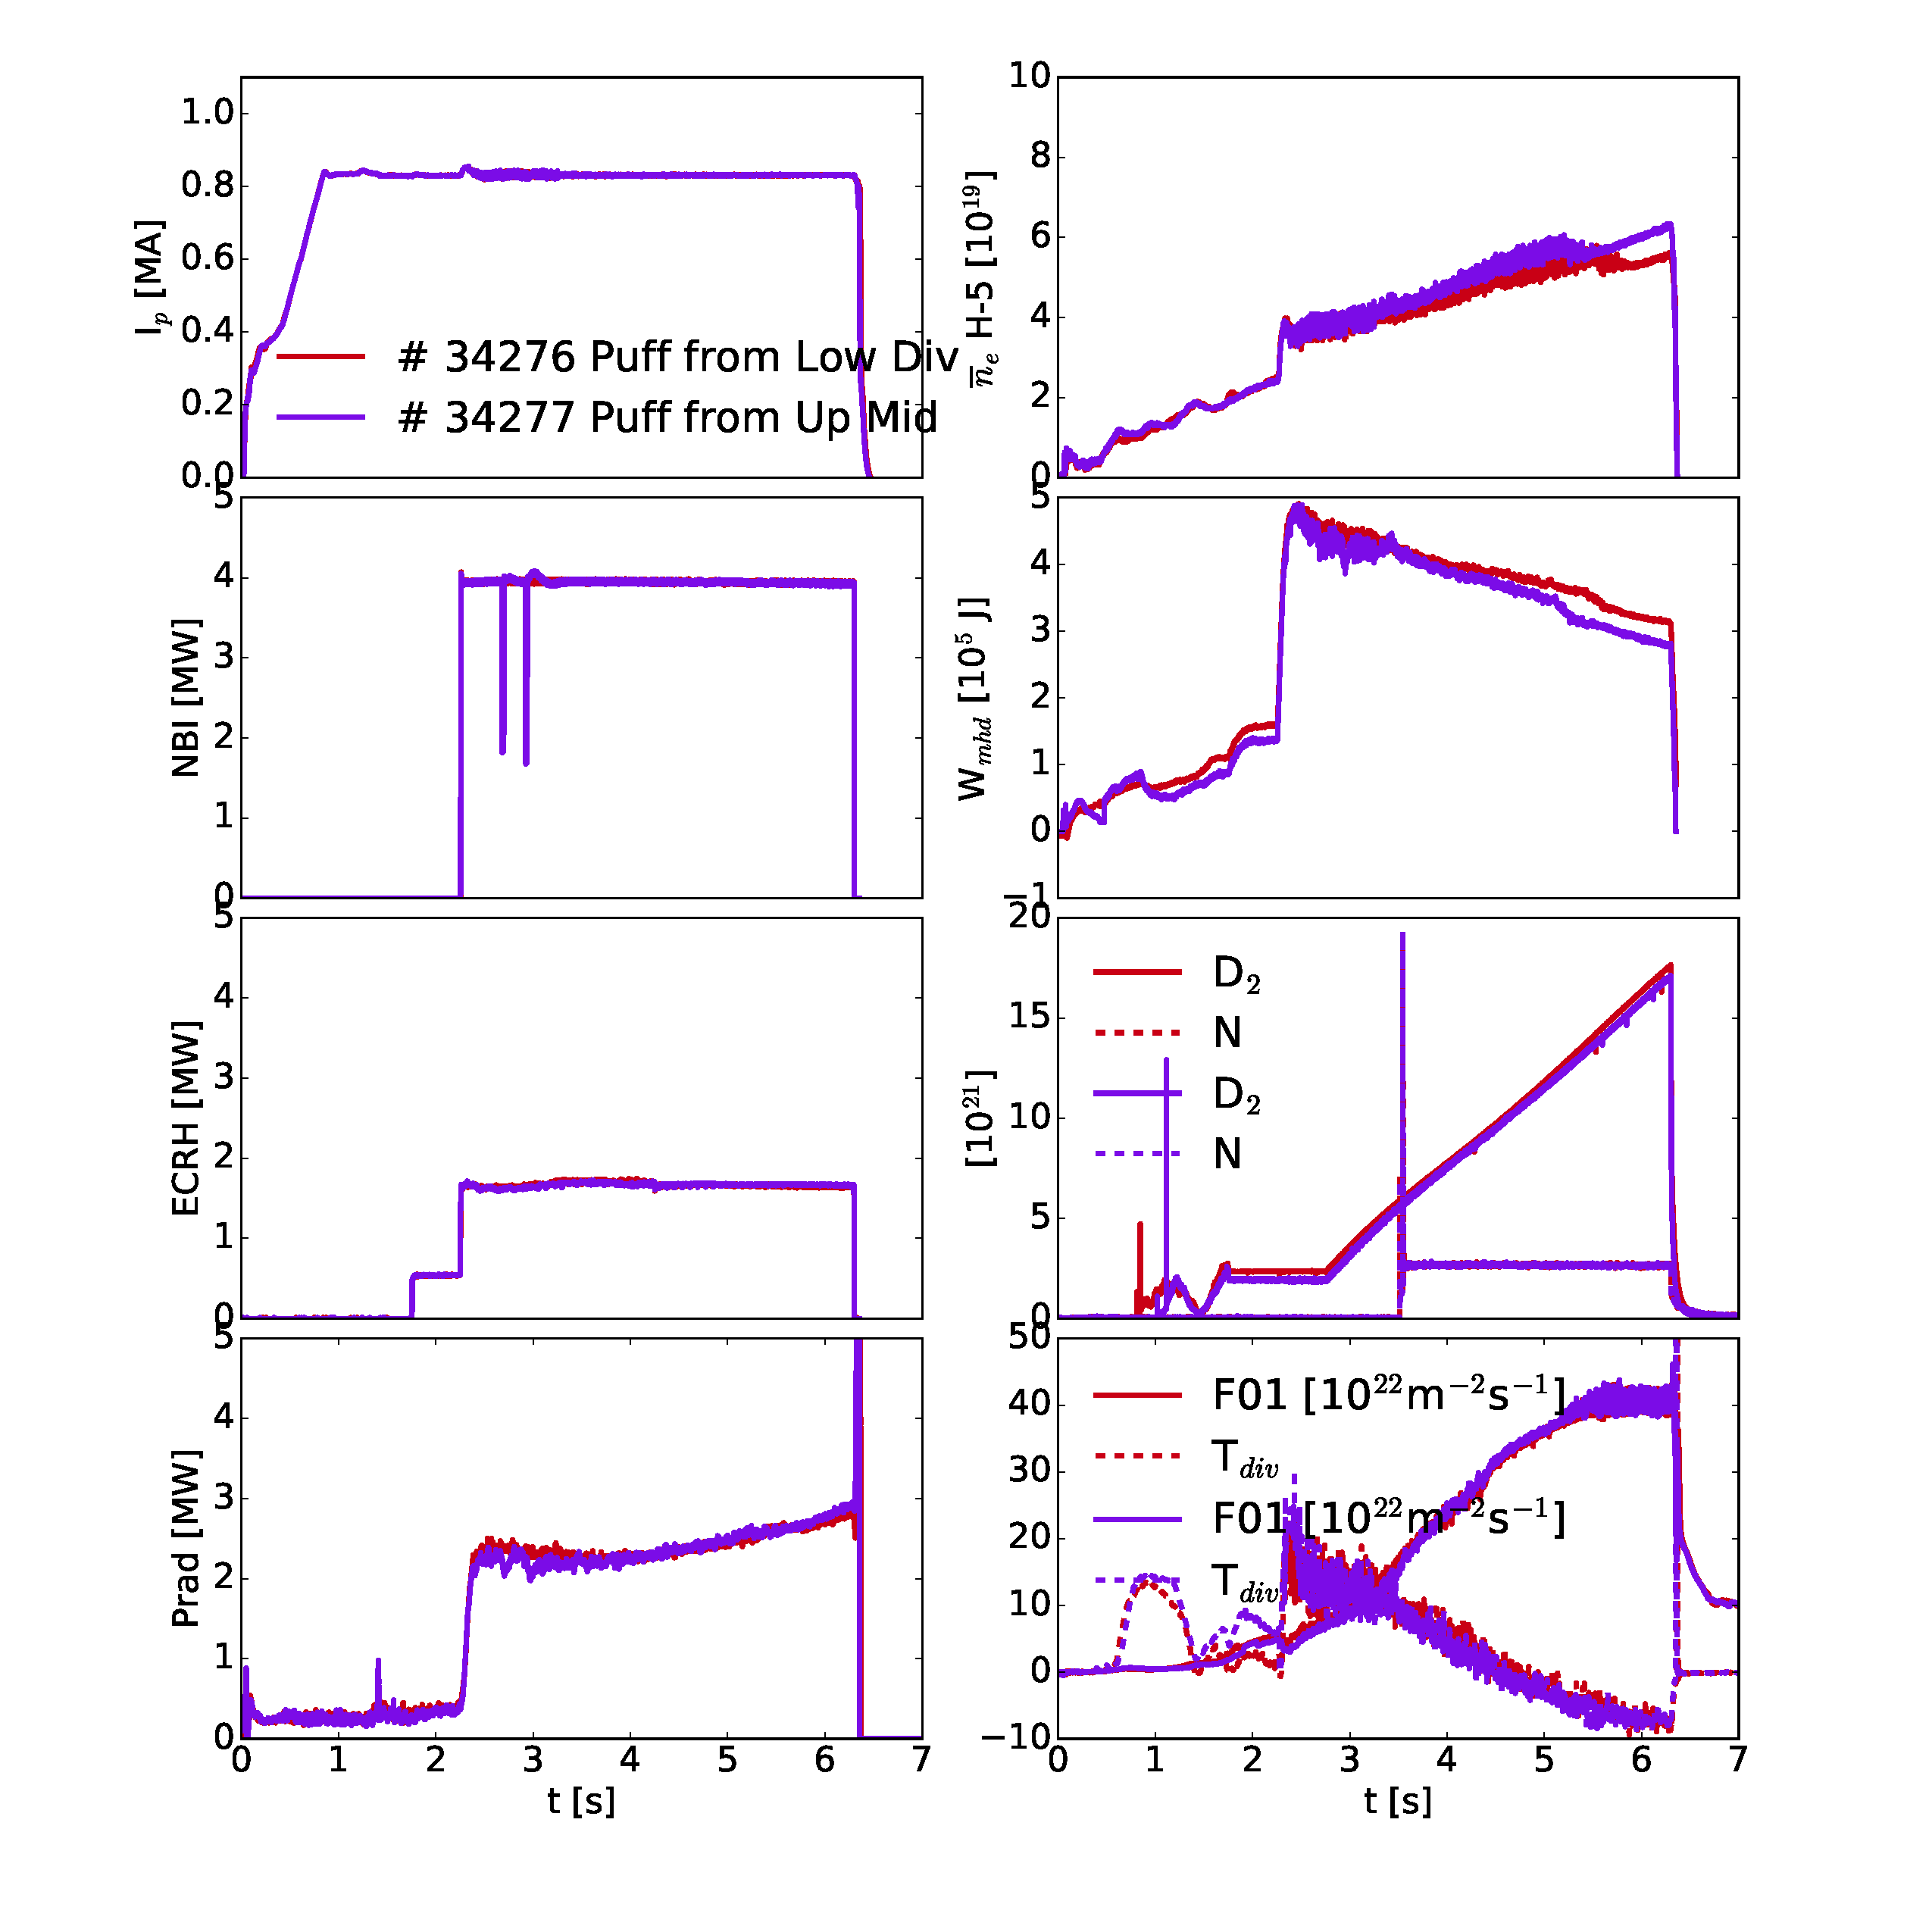
\includegraphics[width=\textwidth]{../../Experiments/AUG/analysis/pdfbox/CompareShot34276_34277}}
  \end{column}
  \begin{column}{0.35\textwidth}
    \begin{itemize}
      \item Reference shot with \textbf{EOC} Shape, 0.8MA, B$_{\phi}$ = -2.5 T, 0.5MW NBI heating,
        fueling in order to keep heating approximately constant during
        the current scan
      \item<2-> The fueling has been reduced at lower current for not
        encountering disruption too early
      \item<3-> Up to 3 seconds 0.6 and 0.8 discharge exibits close
        edge and core density as well as neutral pressure from gauges
        under the dome
      \item<4-> During the discharge complete scan of $\Lambda_{div}$
        from well below to well above 1.
      \item<5> In all the cases the profiles evolve and tends to
        become flatter. Preliminary indication suggest this occurs at
        similar $\Lambda_{div}$
    \end{itemize}
  
  \end{column}
\end{columns}
\end{frame}


\begin{frame}{L-Mode: Current scan at constant $B_{t}$}
\Fontvi
  \vspace{-1cm}
\begin{columns}
  \begin{column}{0.65\textwidth}
    \centering{\includegraphics<1-2>[width=\textwidth]{../../Experiments/AUG/analysis/pdfbox/GeneralIpScanConstantBt}}
    \centering{\includegraphics<3>[width=\textwidth]{../../Experiments/AUG/analysis/pdfbox/EvolutionEdgeProfileConstantBt}}
  \end{column}
  \begin{column}{0.35\textwidth}
    \begin{itemize}
      \item<1-> The fueling has been reduced at lower current for not
        encountering disruption too early
      \item<2-> Up to 3 seconds 0.6 and 0.8 MA discharges exibits close
        edge and core density as well as neutral pressure from gauges
        under the dome
      \item<3> In all the cases the profiles evolve and tends to
        become flatter. Work in progress to evaluate development as a
        function of divertor collisionality $\Lambda_{div}$
    \end{itemize}
  
  \end{column}
\end{columns}
\end{frame}

\begin{frame}{Fluctuations}
  \begin{columns}
\begin{column}{0.5\textwidth}
    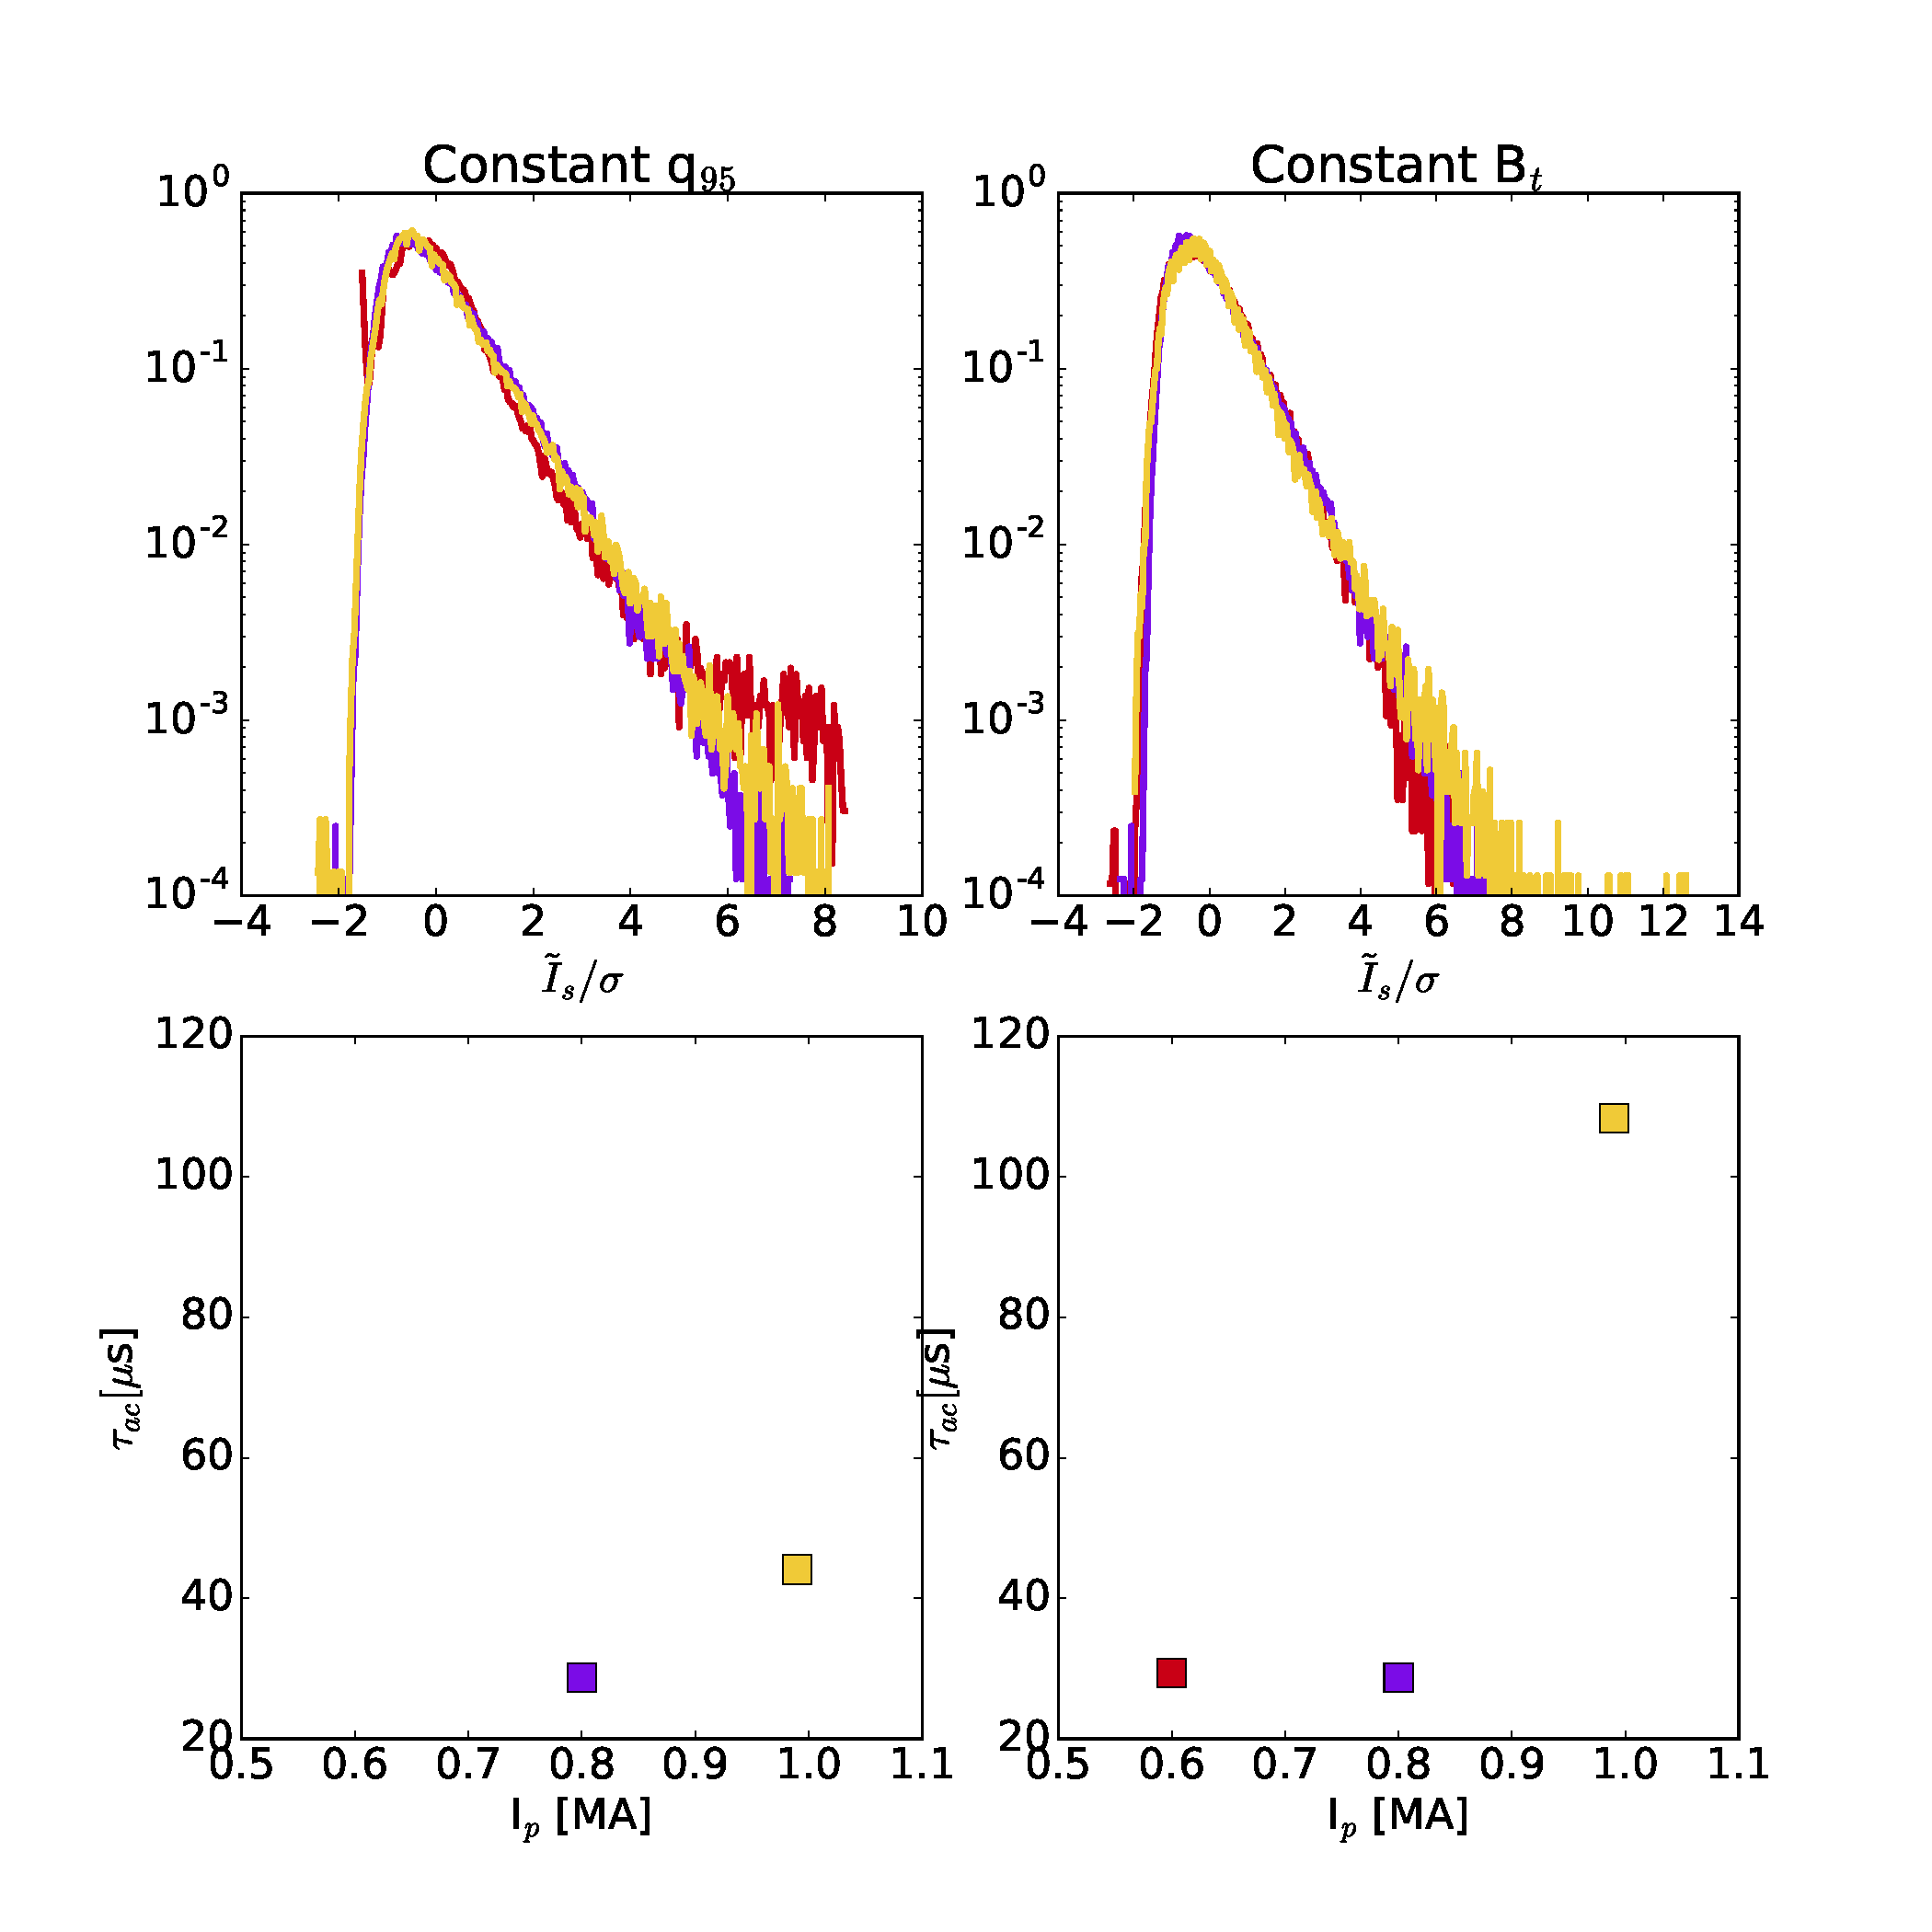
\includegraphics[width=\textwidth]{../../Experiments/AUG/analysis/pdfbox/ScalingAutoCorrelation}
  \end{column}
\begin{column}{0.5\textwidth}
\end{column}
\end{columns}
\end{frame}

\begin{frame}{H-Mode}
\Fontvi
  \vspace{-1cm}
\begin{columns}
  \begin{column}{0.5\textwidth}
    \centering{\includegraphics<1>[width=\textwidth]{../../Experiments/AUG/analysis/pdfbox/Shot34107_GeneralHmod}}
    \centering{\includegraphics<2>[width=\textwidth]{../../Experiments/AUG/analysis/pdfbox/Shot34108_GeneralHmod}}    
    \centering{\includegraphics<3>[width=\textwidth]{../../Experiments/AUG/analysis/pdfbox/DegradedHModeShot34108}}    
    \centering{\includegraphics<4>[width=\textwidth]{../../Experiments/AUG/analysis/pdfbox/Shot34115_GeneralHmod}}    
    \centering{\includegraphics<5>[width=\textwidth]{../../Experiments/AUG/analysis/pdfbox/DegradedHModeShot34115}}    
    \centering{\includegraphics<6>[width=\textwidth]{../../Experiments/AUG/analysis/pdfbox/CompareShot33478_34115}}    
  \end{column}
  \begin{column}{0.5\textwidth}
    \begin{itemize}
      \item<1-> \textbf{EOC} shape, initially with 2MW NBI + 1.4MW ECRH
        density ramp without N seeding
      \item<2-> We increase the NBI power up to 4MW with the same ECRH
        adding N in feedforward
      \item<3-> We end up in a degraded H-Mode with all the 4
        phases. Fluctuations from MEM available in all the phases
      \item<4-> We reduce the N dosing finding a proper scenario
        \alert{but without cryopumps}
      \item<5-> In this cases we still encounters a degraded H-Mode but
        without all the phases
      \item<6-> With respect to the reference we achieve higher power
        and higher neutral pressure in the divertor. We will need to
        adjust once the cryopump will operate in the next session 
    \end{itemize}
  \end{column}
\end{columns}
\end{frame}

\begin{frame}{Fast particle accelleration}
  \Fontvi
  \begin{columns}
    \begin{column}{0.4\textwidth}
      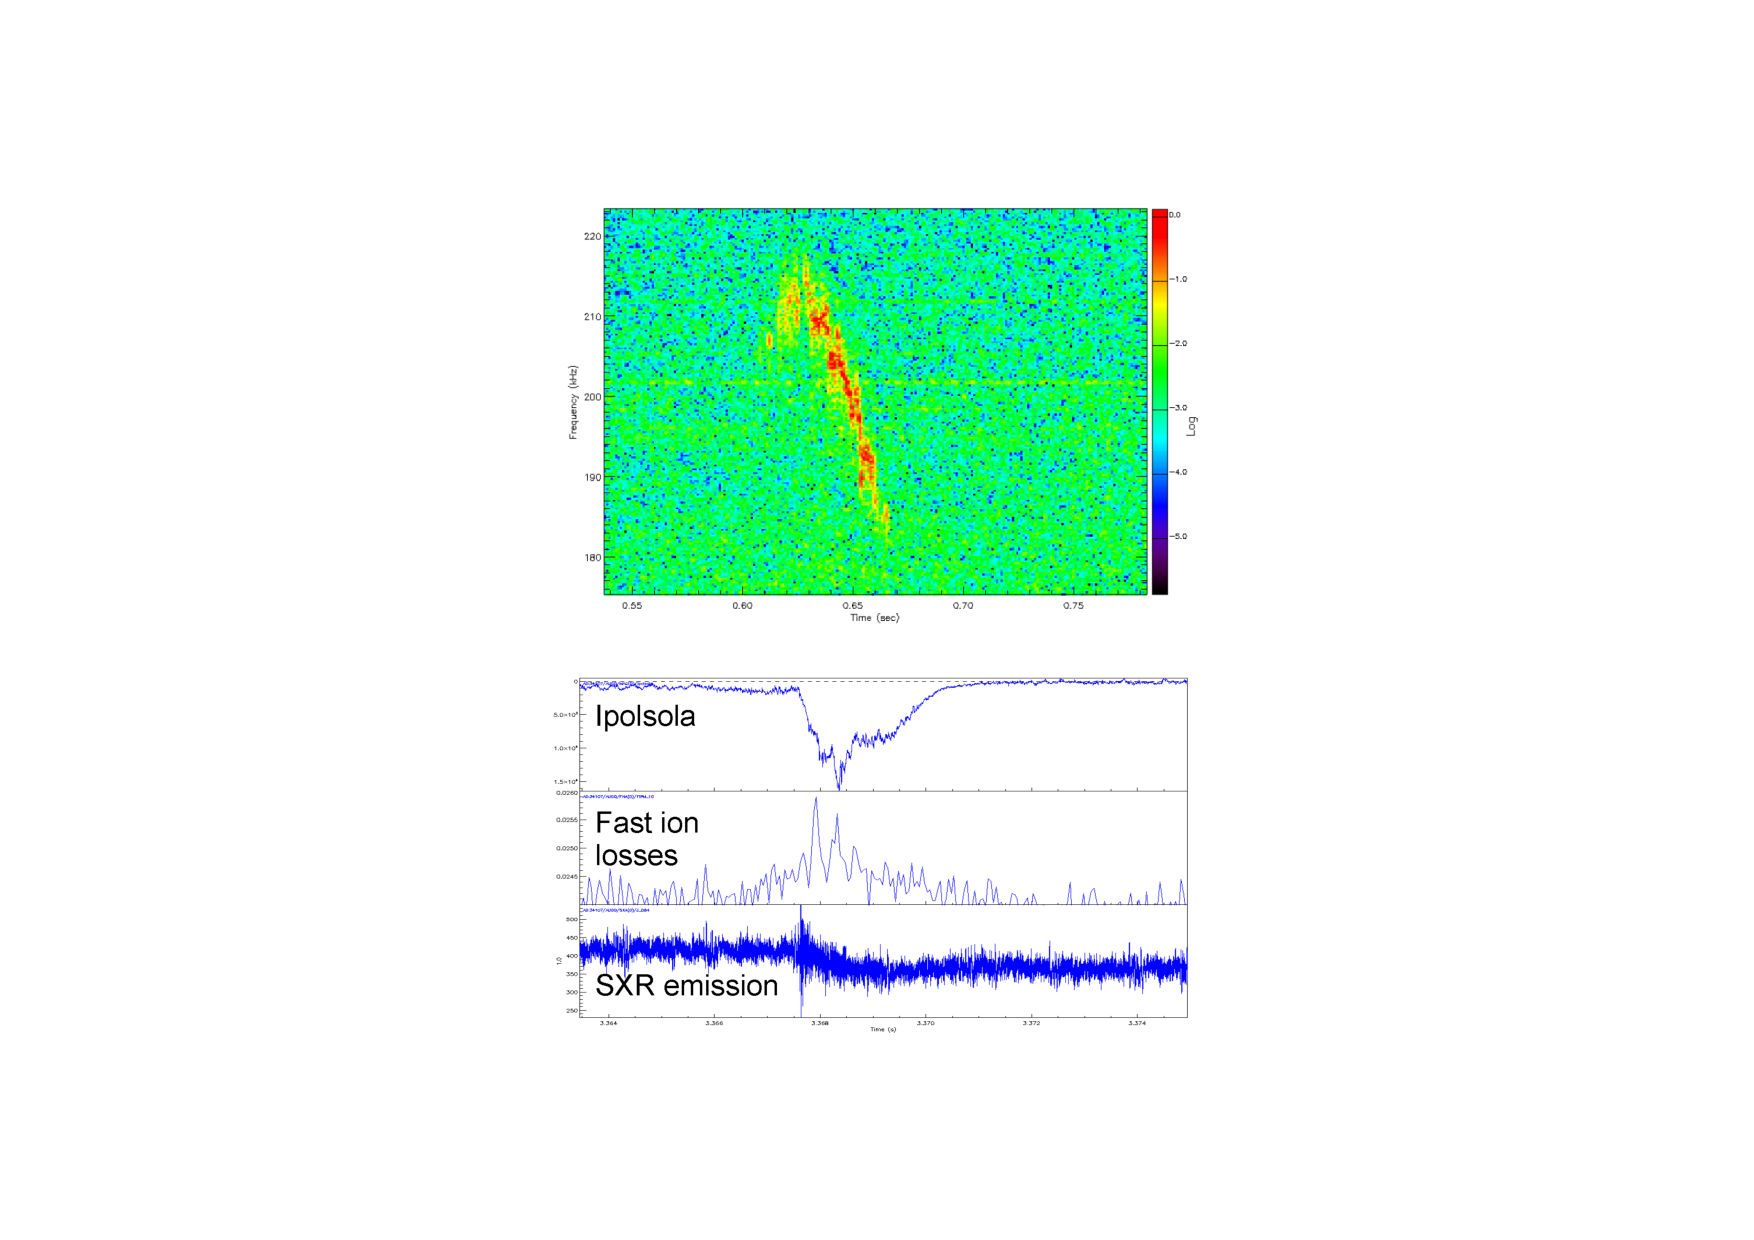
\includegraphics[width=\textwidth]{../../Experiments/AUG/analysis/pdfbox/KenAnalysis} \\
      \textcolor{red}{K. McClements \& J. Galdon-Quiroga}
    \end{column}
    \begin{column}{0.6\textwidth}
    \begin{itemize}
\item L-mode shots: no evidence of electron or ion acceleration during flat-top, but TAE excitation (top) \&
  neutron time traces during current ramp-up in three shots suggest bulk ion acceleration
\item H-mode shots: many examples found of SXR spikes from plasma edge at start of ELMs $\rightarrow$ electron acceleration),
  although enhancements are less dramatic than in earlier H-mode pulses with lower pedestal $\nu^{*}$ (lower plot)
\item ELMs also linked to enhanced fast ion losses, as in previous H-mode pulses –
  not yet clear whether beam ions are accelerated during ELMs, but fast ion loss detector settings will be optimised in remaining pulses of this experiment
\end{itemize}
\end{column}
\end{columns}
\end{frame}

\end{document}

